\documentclass[fontset=mac]{ctexbeamer}
\usepackage{graphicx}
\usepackage{longtable}
\usepackage{wrapfig}
\usepackage{rotating}
\usepackage[normalem]{ulem}
\usepackage{amsmath}
\usepackage{amssymb}
\usepackage{capt-of}
\usepackage{hyperref}
\author{董晨阳}
\institute{风保系 1800015446}
\date{\today}
\title{我国资本市场债券违约特征分析}
\usepackage[style=gb7714-2015ay]{biblatex}
\usetheme{CambridgeUS}
\def\ernest{notes see \url{https://ernestdong.github.io/notes}}
\addbibresource{reference.bib}
\begin{document}
\setbeamertemplate{bibliography item}{}
\setbeamertemplate{bibliography entry article}{}
\setbeamertemplate{bibliography entry title}{}
\setbeamertemplate{bibliography entry location}{}
\setbeamertemplate{bibliography entry note}{}
\setbeamertemplate{caption}[numbered]
\AtBeginSection[]
{
	\begin{frame}
		\tableofcontents[currentsection,currentsubsection,sectionstyle=show/shaded,subsectionstyle=show/show/hide,subsubsectionstyle=show/show/show/hide]
	\end{frame}
}
\maketitle
\begin{frame}{目录}
	\tableofcontents[hideallsubsections]

\end{frame}

\section{我国债券市场历史违约概述}
% !TeX root = main.tex
\subsection{债务违约一览}
\begin{frame}{债券违约史}
	债券违约是资本市场中的正常现象
	\begin{itemize}
		\item 2014年,超日债违约打破“刚兑”
		\item 2020年,永煤、华晨违约打破“国企信仰”
		\item 2021年,近期地产债违约大潮
		\item 未来城投债压力
	\end{itemize}
\end{frame}
\begin{frame}{债券违约:分行业}
	\begin{table}[]
		\resizebox{\columnwidth}{!}{%
			\begin{tabular}{llllll}
				\hline
				\multicolumn{1}{c}{\textbf{行业}} & \multicolumn{1}{c}{\textbf{违约债券只数}} & \multicolumn{1}{c}{\textbf{违约债券余额(亿元)}} & \multicolumn{1}{c}{\textbf{余额违约率(\%)}} & \multicolumn{1}{c}{\textbf{违约发行人个数}} & \multicolumn{1}{c}{\textbf{发行人个数违约比率(\%)}} \\ \hline
				信息技术业                        & 36                                        & 423.72                                          & 21.13                                       & 4                                           & 10.00                                               \\
				批发和零售贸易                    & 65                                        & 679.34                                          & 8.93                                        & 15                                          & 9.09                                                \\
				制造业                            & 164                                       & 1,165.98                                        & 8.04                                        & 58                                          & 19.66                                               \\
				农、林、牧、渔业                  & 2                                         & 11.50                                           & 2.63                                        & 2                                           & 9.52                                                \\
				房地产业                          & 27                                        & 267.48                                          & 2.15                                        & 9                                           & 3.57                                                \\
				综合类                            & 75                                        & 705.08                                          & 1.27                                        & 20                                          & 2.55                                                \\
				交通运输、仓储业                  & 34                                        & 350.60                                          & 0.96                                        & 12                                          & 5.08                                                \\
				采掘业                            & 18                                        & 96.11                                           & 0.92                                        & 5                                           & 7.69                                                \\
				建筑业                            & 41                                        & 415.44                                          & 0.61                                        & 11                                          & 0.56                                                \\
				传播与文化产业                    & 1                                         & 3.00                                            & 0.61                                        & 1                                           & 3.70                                                \\
				社会服务业                        & 8                                         & 66.69                                           & 0.39                                        & 6                                           & 1.55                                                \\
				电力、煤气及水的生产和供应业      & 5                                         & 37.98                                           & 0.20                                        & 3                                           & 1.18                                                \\
				金融、保险业                      & 2                                         & 9.99                                            & 0.02                                        & 2                                           & 0.34                                                \\
				\textbf{合计}                     & \textbf{478}                              & \textbf{4,232.91}                               & \textbf{1.45}                               & \textbf{148}                                & \textbf{2.91}                                       \\ \hline
			\end{tabular}
		}
		\caption{违约境内债行业分布\footnote{数据来源:wind}}
		\label{fig:default_indus}
	\end{table}
	如表 \ref{fig:default_indus}所示,违约债券最多的行业是制造业,其次是综合类、批发和零售贸易。近期热点的主要是房地产类,2021年来实质违约、展期的房地产企业包括但不限于重庆协信、华夏幸福、四川蓝光、花样年、新力控股、当代置业、鑫苑置业、中国奥园、阳光城、佳兆业、恒大、阳光100等
\end{frame}

\begin{frame}{违约债:分地域}
	\begin{columns}
		\column{0.6\linewidth}
		\begin{figure}
			\centering
			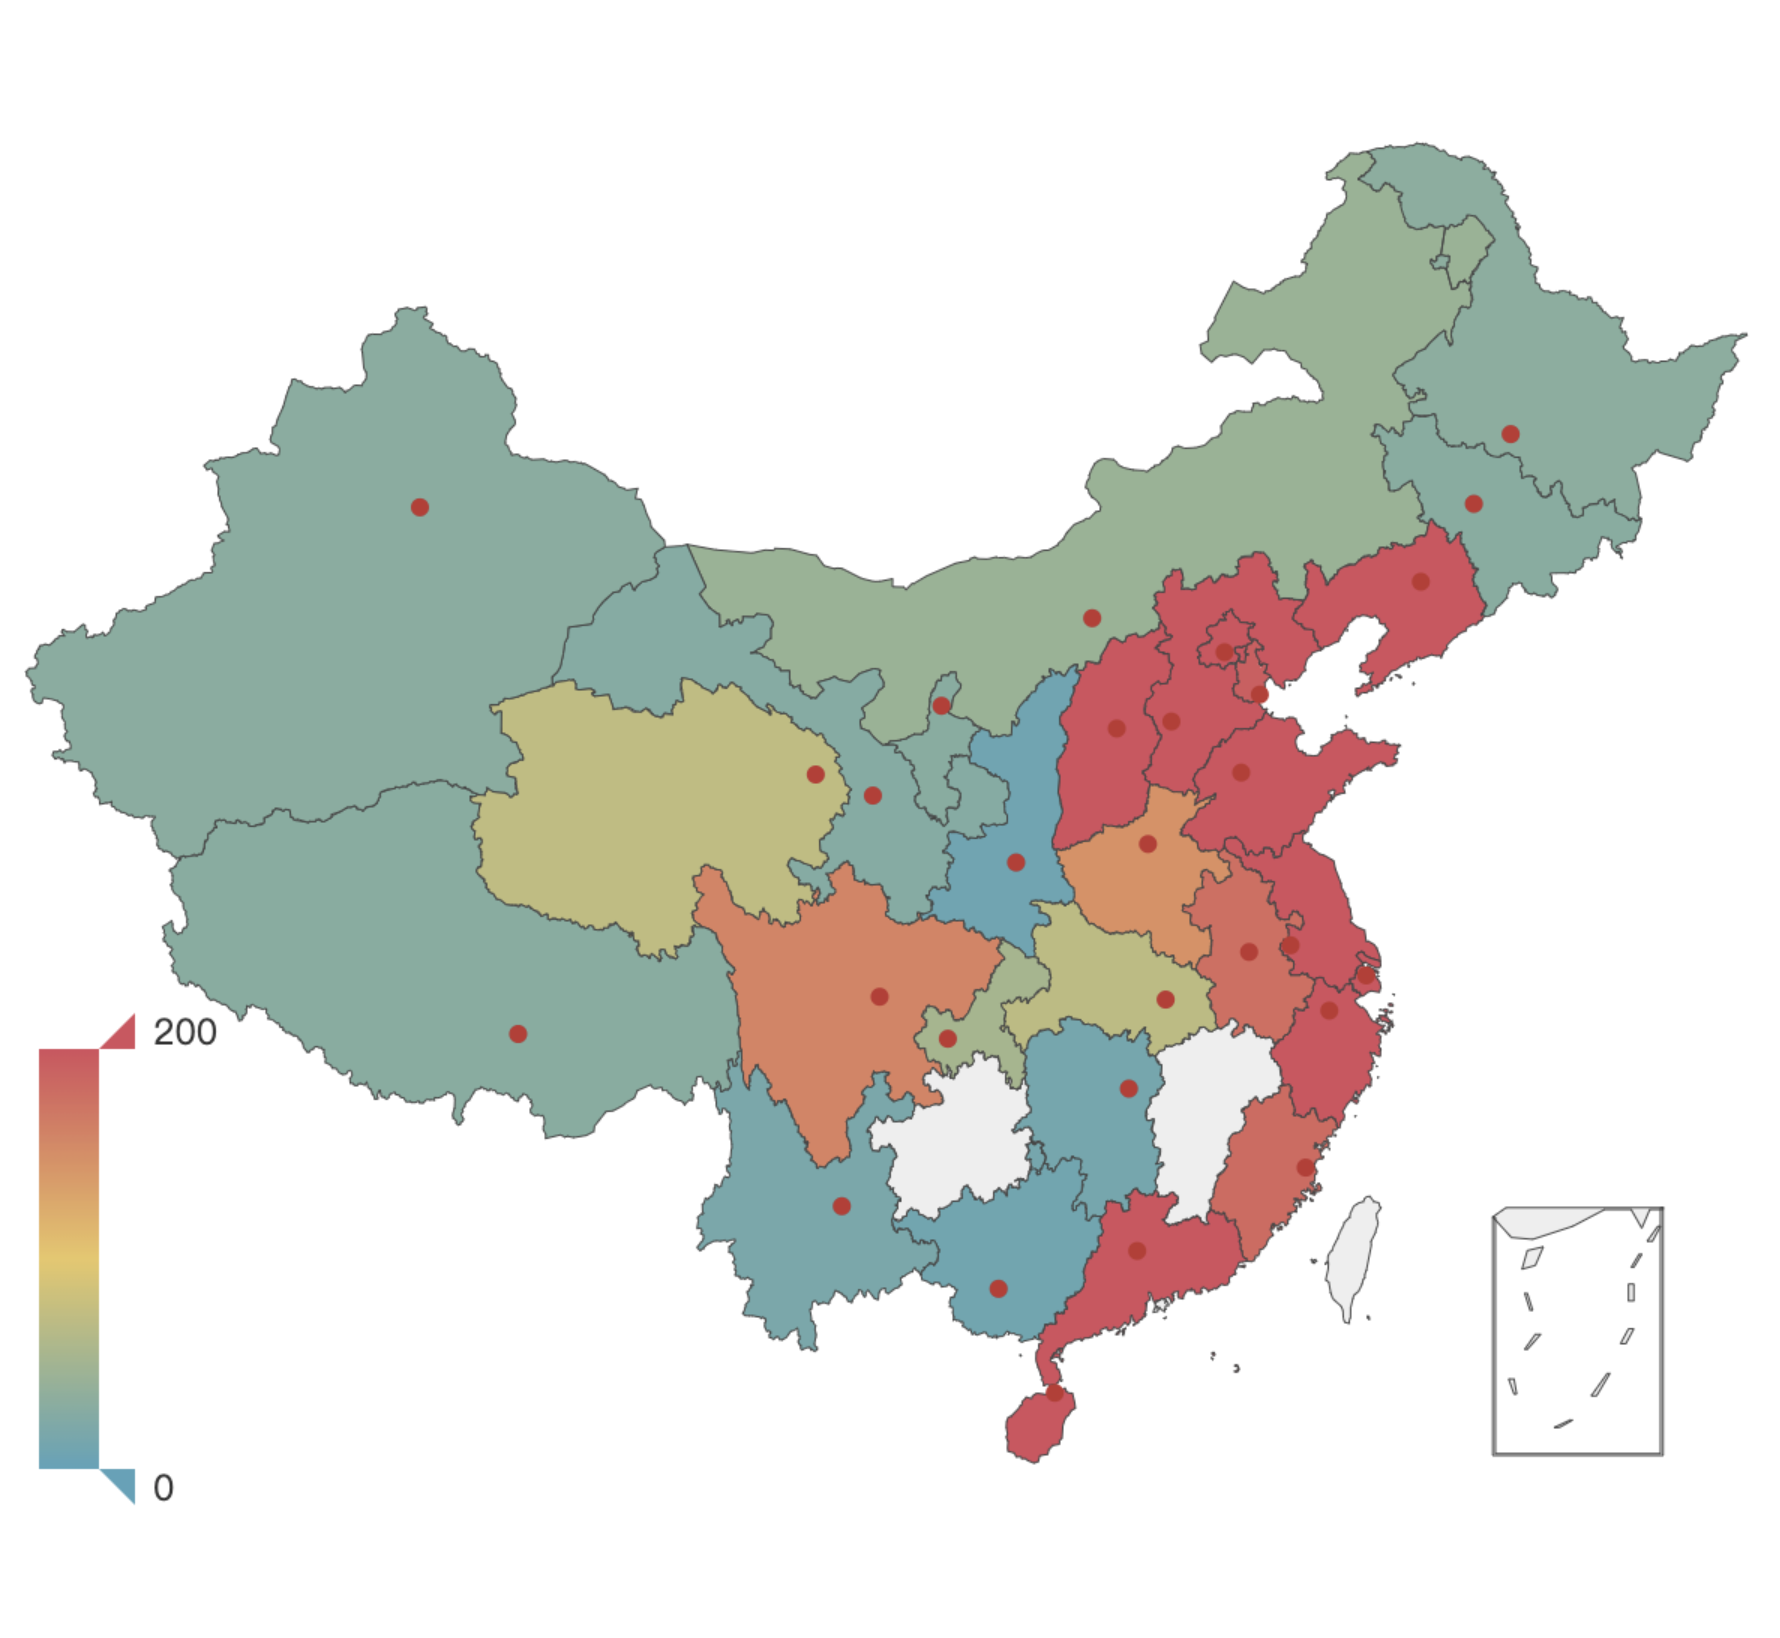
\includegraphics[width=\linewidth]{lib/default_by_geo.png}
			\caption{违约债券余额}
			\label{fig:defaultGeo}
		\end{figure}
		\column{0.35\linewidth}
		北京以违约债券105只、1,212.40亿元占第一位。

		一方面经济落后地区违约风险较大,一方面经济较好的地区企业发债数量较多可能导致违约金额较大,图\ref{fig:defaultGeo}显示出后一种作用较强。
	\end{columns}
\end{frame}
\subsection{债务违约后果}
\begin{frame}{对持有人}
	\begin{columns}[c]
		\column{0.4\linewidth}
		对于债券人持有人而言,不仅面临债券违约带来的本金损失,还将引发一系列问题。
		\begin{itemize}
			\item 机构面临赎回带来的流动性压力
			\item 结构化发行,或引发交易纠纷
			\item 投入较长的求偿时间,清偿率平均越20\%
		\end{itemize}
		\column{0.5\linewidth}
		\begin{figure}
			\centering
			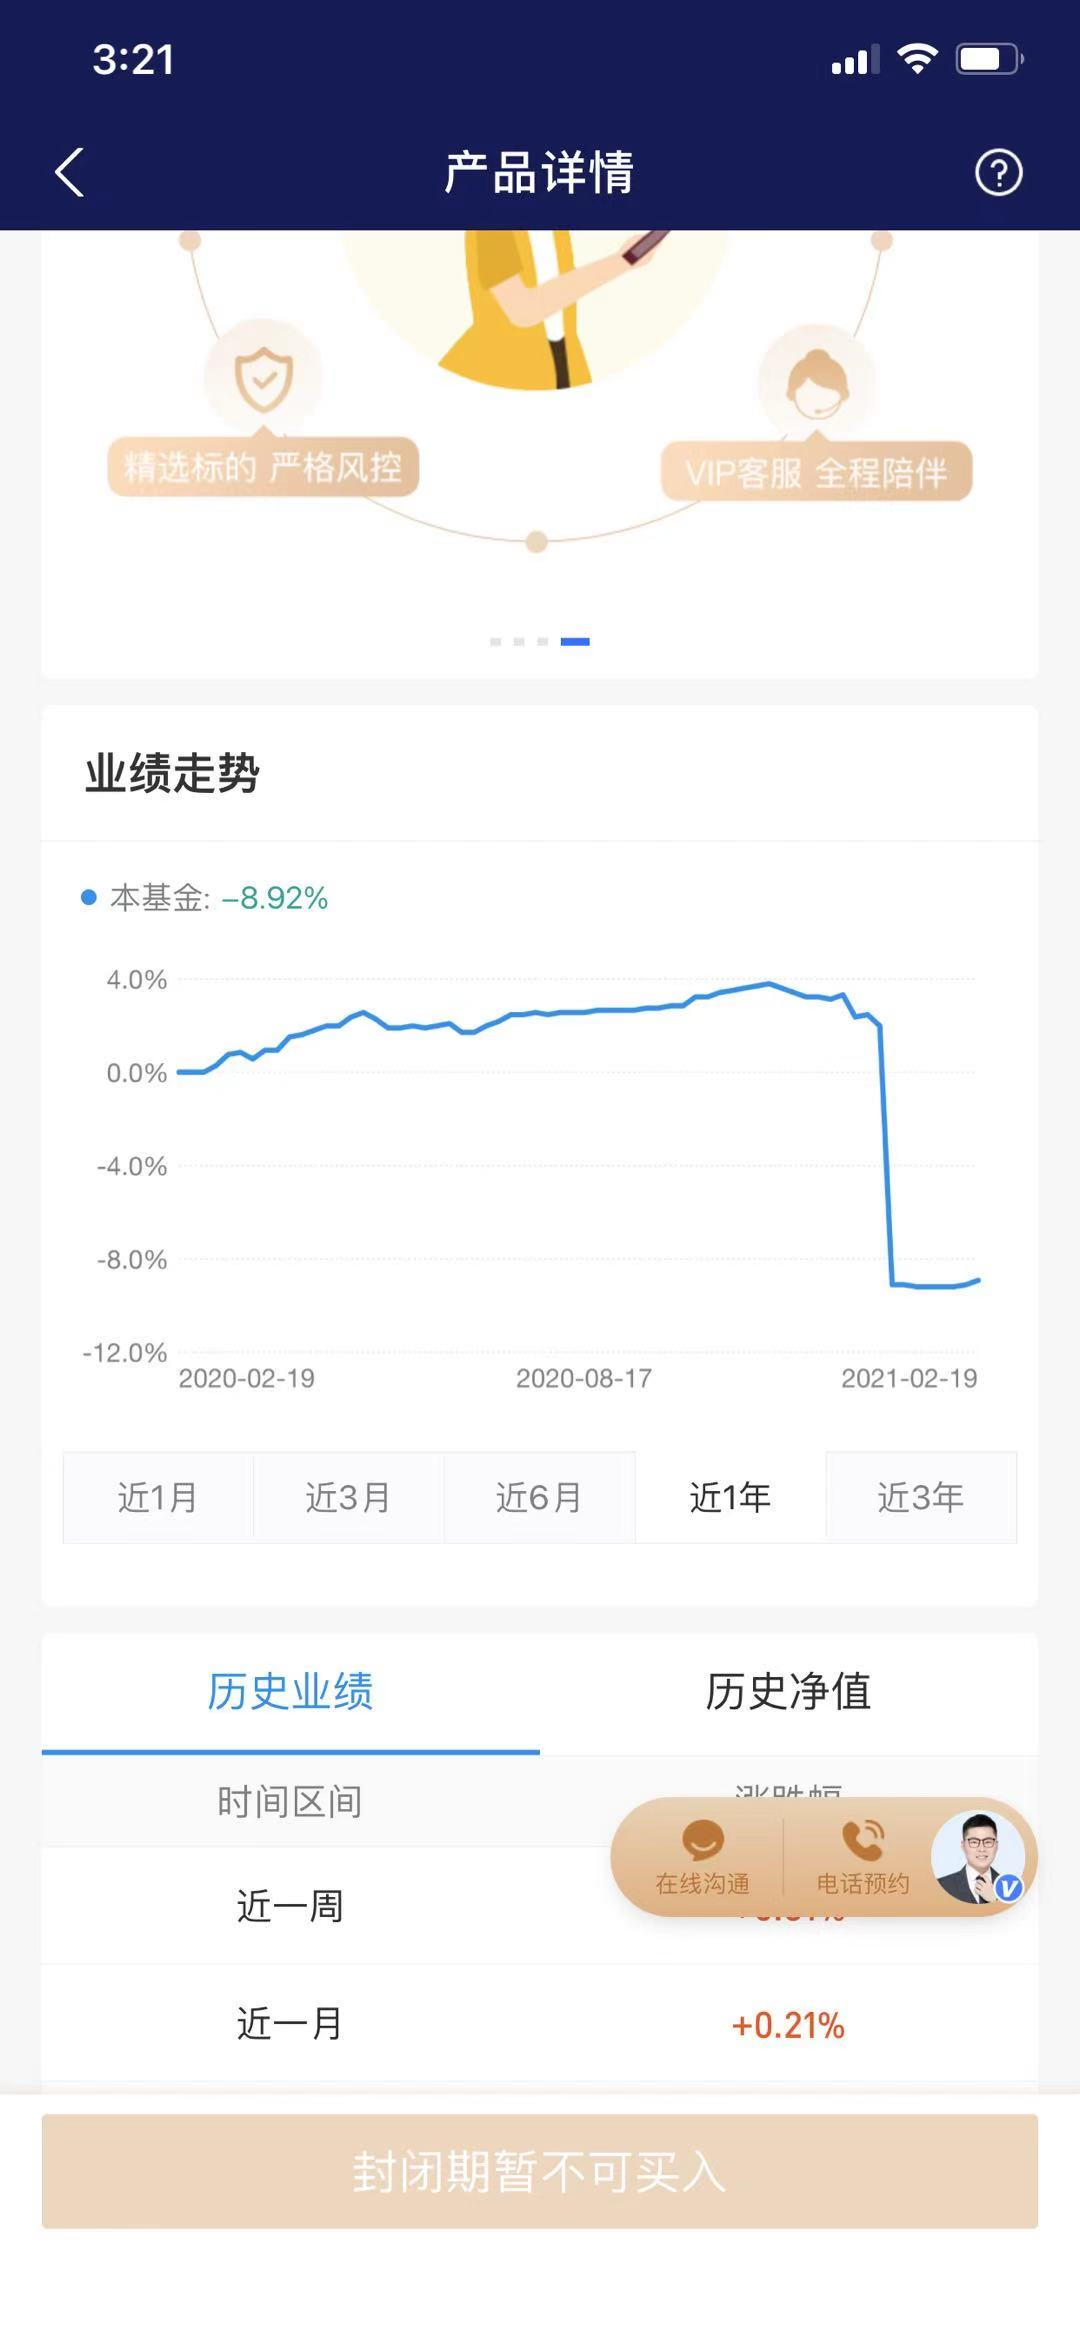
\includegraphics[width=0.6\linewidth]{lib/jsfund.jpg}
		\end{figure}
	\end{columns}
\end{frame}
\begin{frame}{对发行人}
	\begin{itemize}
		\item 削弱外部融资功能
		\item 交叉违约条款引发偿债压力急升
		\item 负面事件引发内部管理层动荡
		\item 影响企业的生产经营
	\end{itemize}
\end{frame}
\begin{frame}{外部性}
	\begin{columns}[c]
		\column{0.5\linewidth}
		企业信用风险可能会传染,可能是由于股权、业务/地区相似或投资人心理,引发进一步的危机。\newline
		2020年11月10日,永煤违约之后,一级市场上河南方面拟发行的5只债券没有一只发行成功,一个月内累计1000亿信用债取消发行;二级市场上清控、豫能化债券价格闪崩,并最终违约。
		\column{0.5\linewidth}
		\begin{figure}
			\centering
			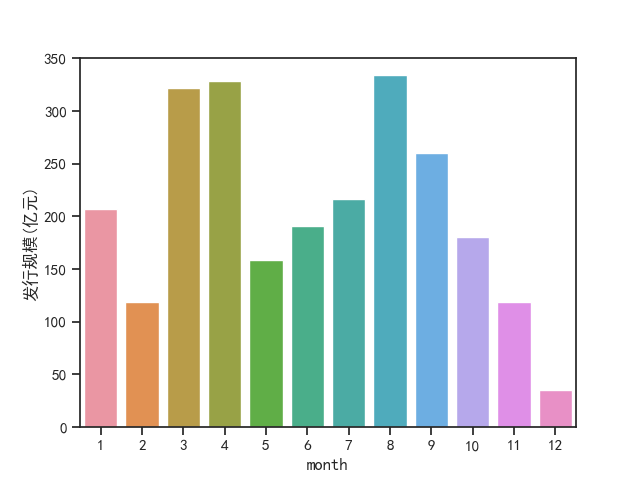
\includegraphics[width=\linewidth]{lib/henan.png}
			\caption{国企信仰崩塌,河南信用债发行骤减}
		\end{figure}
	\end{columns}
\end{frame}


\section{文献综述}
% !TeX root = main.tex
\subsection{信用利差}
\begin{frame}{影响因素}
	\begin{itemize}
		\item 信用评级\cite{陈关亭2021多重信用评级与债券融资成本}\cite{黄小琳2017债券违约对涉事信用评级机构的影响——基于中国信用债市场违约事件的分析}\cite{寇宗来2015中国的信用评级真的影响发债成本吗}\cite{寇宗来2021私有信息}
		\item 公司治理\cite{常莹莹2019环境信息透明度与企业信用评级}
		\item 市场流动性\cite{钟宁桦2018散户投资者如何影响债券价格}
		      % \item 流动性溢价
		      % \item 跨市场流动性
		\item 宏观政策\cite{韩鹏飞2015政府隐性担保一定能降低债券的融资成本吗}\cite{汪莉2015政府隐性担保}
		      \begin{itemize}
			      \item 财政政策\cite{梅冬州2021财政扩张}、
			      \item 货币政策\cite{王博2019货币政策不确定性}
			            宏观环境\citet{bai2019common}
		      \end{itemize}
	\end{itemize}
	\ernest{}
\end{frame}

\subsection{风险传染}
\begin{frame}{传染路径}
	在美国,违约风险传染主要是宏观层面和微观层面的 \citet{azizpour2018exploring}
	\begin{itemize}
		\item 系统性风险\cite{苟文均2016债务杠杆与系统性风险传染机制——基于}
		\item 非系统性风险\cite{钟辉勇2016城投债的担保可信吗}
	\end{itemize}
	\ernest{}
\end{frame}


\section{理论分析}
\subsection{宏观因素}
\begin{frame}{政策与环境}
	货币政策、财政政策
	\begin{itemize}
		\item 疫情
		\item 贸易战
		\item 经济下行 \citet{bali2021macroeconomic}
	\end{itemize}
\end{frame}


\begin{frame}{市场流动性}
	市场流动性偏紧,企业正常融资无法接续。如永煤违约之后相似主体如清控、紫光、冀中能源等发债遇到困难,最终部分主体走向违约。
\end{frame}

\subsection{中观因素}
\begin{frame}{行业景气和行业政策}
	房地产政策、光伏补贴政策都可能影响企业违约。

	顺周期行业中可能因为行业景气循环判断失误,经营出现问题,影响偿债能力。
\end{frame}
\begin{frame}{地域}
	区域风险传染,可能的路径有股权、人事、地区互保等情况,一荣俱荣一损俱损。
\end{frame}
\subsection{微观因素}
\subsubsection{公司层面}
\begin{frame}{公司治理}
	\begin{itemize}
		\item 高管变动\cite{林晚发2018高管任职经历的得与失}
		\item 母子关系
		\item 客户集中度\cite{王雄元2017客户集中度与公司债二级市场信用利差}
	\end{itemize}
\end{frame}

\begin{frame}{经营}
	\begin{itemize}
		\item 业绩巨亏
		\item 非标违约
		\item 对外担保
		\item 股权质押
		\item 客户集中度 \citep{王雄元2017客户集中度与公司债二级市场信用利差}
	\end{itemize}
\end{frame}

\begin{frame}{财务}
	\begin{itemize}
		\item 杠杆\cite{王永钦2019杠杆率如何影响资产价格}
		\item 营业收入
		\item 货币资金
	\end{itemize}
\end{frame}

\begin{frame}{发行人主观意愿}
	难以量化。

	\begin{quote}
		永城煤电在2020年10月20日发行“20永煤MTN006”、账面仍有大量货币资金时选择“20永煤SCP003”违约逃废债。

		花样年在账面留有大量现金时因行业景气结束选择躺平放弃履约。
	\end{quote}

\end{frame}
\subsubsection{债项层面}
\begin{frame}{债券分类}
	我国信用债针对发行面向对象可分为公募债和私募债。针对公募债和私募债,监管要求的信息披露、发行条件等也有所不同。

	因此相似期限的中期票据(公募债的一种)违约率通常比定向债务融资工具(私募债)高。
\end{frame}
\begin{frame}{收益率、折算率、评级}
	高收益率伴随而来的是高风险。正是因为承担了较大的风险,投资者才会要求债券给予较大的收益率补偿。
\end{frame}
% \begin{frame}{标准券折算率}
% 不透明,放弃
% \end{frame}


\section{实证检验}
% !TeX root = main.tex
\subsection{违约定义}
\begin{frame}{展期不算违约?}
	近几个月来,房地产企业暴雷不断,有人因此提出“展期不算违约”,阳光城、奥园等地产企业及恒大上游供应商南通三建等纷纷进行展期的操作。

	但展期延长还款本质上仍然违反了债券签订时的合同,侵害投资者利益,并且展期最后是否能真正还款仍有很大变数。因此我们认为展期也算作违约。类似的,所谓“技术性违约”,我们也认为属于违约。

	此外,花式躲避违约的方式还有“场外兑付”。历史上看,选择过“场外兑付”的中融新大、山东如意最终都无可挽回的走向了公开市场债券违约。“场外兑付”能否保证投资者利益、避免交叉违约作用存疑。并且不通过交易所直接将利息付给投资者数额不会披露,不一定足额付息,显然违反了债券合同成立时的规则。因此我认为“场外兑付”也算违约。
	\begin{quote}
		恒大地产日公告称,已通过场外方式协商解决关于9月23日到期的“20恒大04”债劵到期利息,该债劵利息共计约2.32亿元。
	\end{quote}
\end{frame}
\begin{frame}{评级}
	\small{\small {尽管\citet{梅冬州2021财政扩张} 论证了机构机构投资者将评级机构的债券评级作 为投资门槛条件,而在做具体决策时则主要通过自己的内部评级和定价分析体系,是因为评级机构评级失真。

			评级机构事前很难公正评级,很多情况下事后才下调评级。但反过来说,下调评级通常包含着信用问题已经比较严重了的信息。因此我们会关注评级是否下调,而不关注评级具体数值和上升的情况。}}
	\begin{figure}
		\centering
		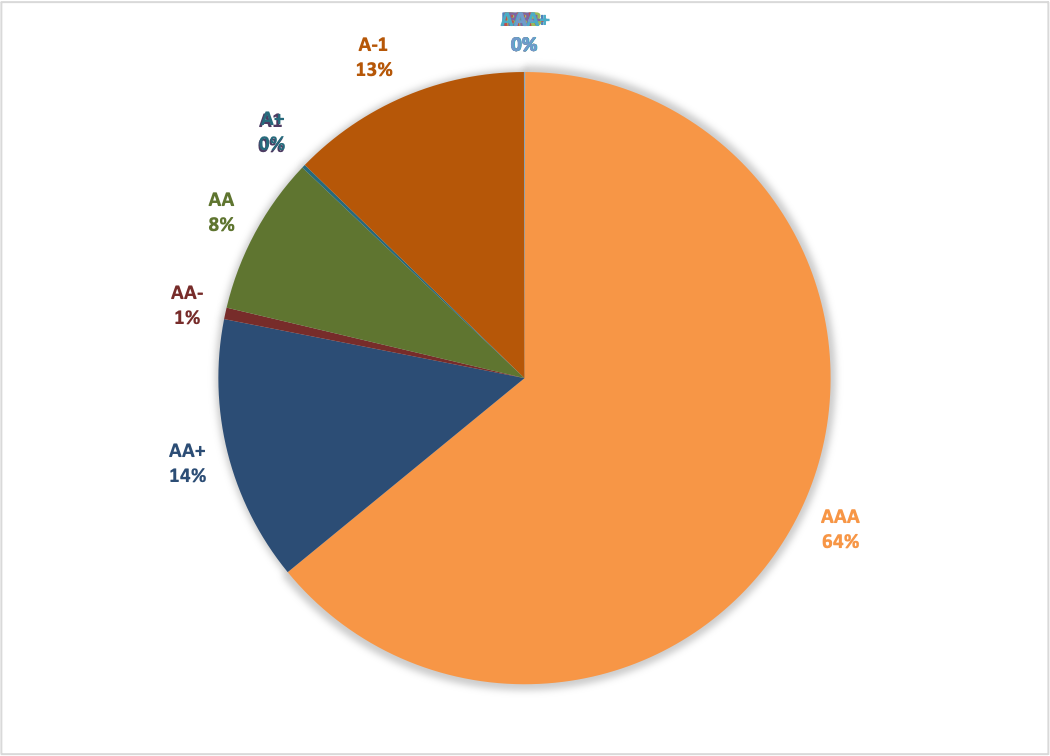
\includegraphics[width=0.6\linewidth]{lib/rating.png}
		\caption{2014年以来评级分布(按金额计)}
	\end{figure}
\end{frame}
\subsection{数据来源及分析}
\begin{frame}
	主要数据来自于 wind 数据库。

	描述性统计 TBA
\end{frame}
\subsection{Logit回归检验}
\label{Logit}
\begin{frame}{回归}
	控制变量:
	\begin{itemize}
		\item 久期
		\item ?
	\end{itemize}
	回归:
	\begin{equation*}
		DEFAULT = \alpha + \beta_1 X_{macro} + \beta_2 X_{industry} + \beta_3 X_{enterprise} + \beta_4 X_{bond} + \beta_5 Control
	\end{equation*}

\end{frame}
\subsection{机器学习加入非线形因素}
\begin{frame}{随机森林算法}
	首先采用决策树降维,梳理哪些因素可能导致违约,并和节\ref{Logit}对比。

	随机森林需要的样本量相对较小,结果比较稳健。

	但采用随机森林方法,结果无法解释。训练结果与节\ref{Logit}比对。
\end{frame}


\section{结论}
\begin{frame}{结论}
	TBA
\end{frame}


\appendix
\begin{frame}[allowframebreaks]{参考文献}
	\nocite{*}
	\printbibliography[heading=bibliography,title=参考文献]
\end{frame}
\end{document}
